% !TeX root = ../main.tex
% Add the above to each chapter to make compiling the PDF easier in some editors.
\chapter{Introduction}\label{chapter:introduction}
\pagenumbering{arabic}
\setcounter{page}{1}
%introduction
In the early days, the computing system that will serve students of an educational institution will occupy a huge space, require very expensive parts and consume a great amount of power but yet will not produce enough computing power required by the students. These computing systems have nowadays been replaced by a number of processing units, storage hard drives and network devices organized in form of a distributed system that combines resources in a more efficient manner while consuming less resources.
\par \setlength{\parskip}{1em}
Clusters and grids are the two well-known paradigms for distributed systems; paradigms that are the basis for the emergence of cloud-computing in the early 2007, with its main purpose being to achieve the long desire of \textit{computing as utility} \cite{corbato1965introduction}. Cloud Computing environment utilizes virtualization techniques to provide a means of assigning resources to "individual" systems (instances). This makes it possible to deploy a pay-per use business models that allow users to choose what computing resource they need, hence drastically reducing their computing cost. This deployment can be in Public, Private, Hybrid, Community or Virtual Private Cloud models - depending on the need of the user. It could also be a combination of one or more of this models, with service delivery models including Infrastructure-as-a-Service (IaaS), Platform-as-a-Service (PaaS) and Software-as-a-Service (SaaS). The private cloud refers to hardware resources virtualized for internal use. Providers and users of the private cloud platform services are the same, hence the resources for data security and service stability is much more effective compared to that of public clouds. It is important for private cloud owners therefore to know the limits of your private cloud so as to efficiently serve its customers and in-cases of educational institution its students.

\section{OpenStack}
OpenStack is an open source project supervised by the OpenStack Foundation. It takes advantage of technologies like Linux distributions, database systems, messaging queues to facilitate the creation and management of different sets of computing resources, storage and networks via a dashboard. OpenStack consists of individual projects/components that manage multiple services used to process different requests. These OpenStack individual components access control policies, logging services, security monitoring tools, etc.

There has been several definitions of OpenStack, a lot of these definitions try to explain the architecture of OpenStack with regards to the components for building a private, public or hybrid cloud. OpenStack architecture is growing and organized in sections with components added continuously over the past years, with each release adding a new components that provide more services in the IaaS layer \cite{kavanagh2015openstack} and based on this an architecture was proposed. 

\begin{figure}[h]
\centering
\IfFileExists{Images/Image001.jpg}{
    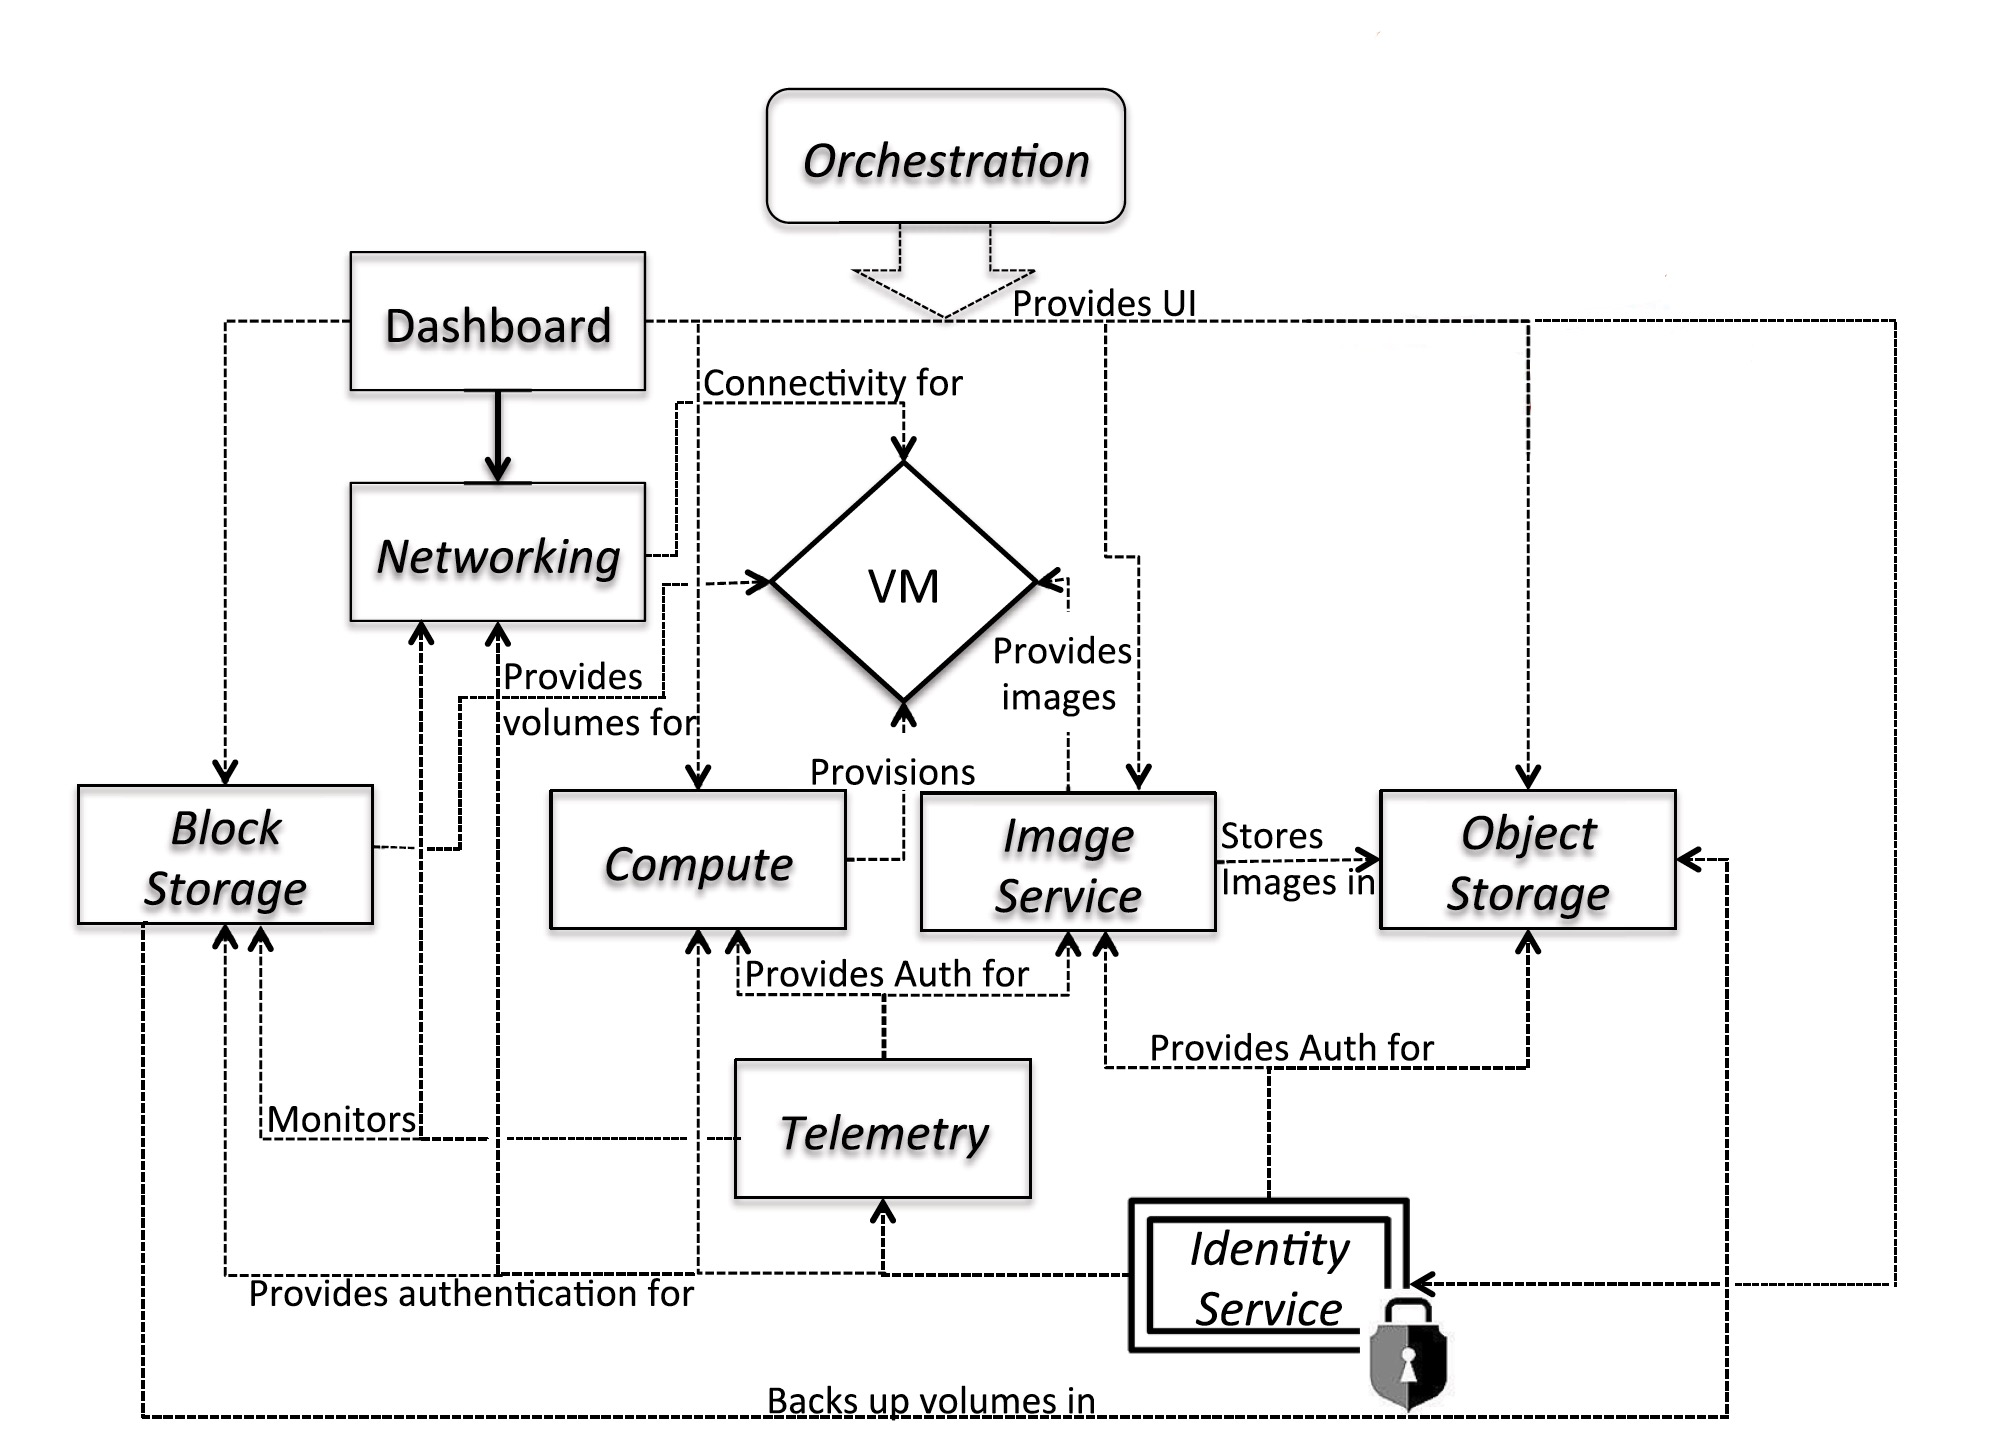
\includegraphics[width=10cm, height=6.5cm]{Images/Image001.jpg}
  }{}
  \caption{Conceptual Architecture of OpenStack adopted from \citeauthor{kavanagh2015openstack} (\citeyear{kavanagh2015openstack}) \cite{kavanagh2015openstack}}
  \label{fig: OpenStack_Arch}
  \floatfoot{\textit{This architecture does not totally explain the components of OpenStack and how they are related to each, it only a conceptual architecture with no detailed explanation as to what is really obtainable with OpenStack in relation to its components}}
\end{figure}

Unlike the architecture in \citeauthor{kavanagh2015openstack}, \citeyear{kavanagh2015openstack} \cite{kavanagh2015openstack}, the OpenStack documentation \cite{OpenStackBlog} explains that OpenStack utilizes a \textit{"modular architecture"} to showcase the set of core services that simplifies scalability and elasticity as core design assumptions. The dashboard contains every other service available with OpenStack but these services can be only accessed through the identity service - after the identity service has identified the user as either an administrator, user or an operator. Identities that are nevertheless set from the dashboard.

\begin{figure}[h]
\centering
\IfFileExists{Images/OpenStack_Architecture.jpg}{
    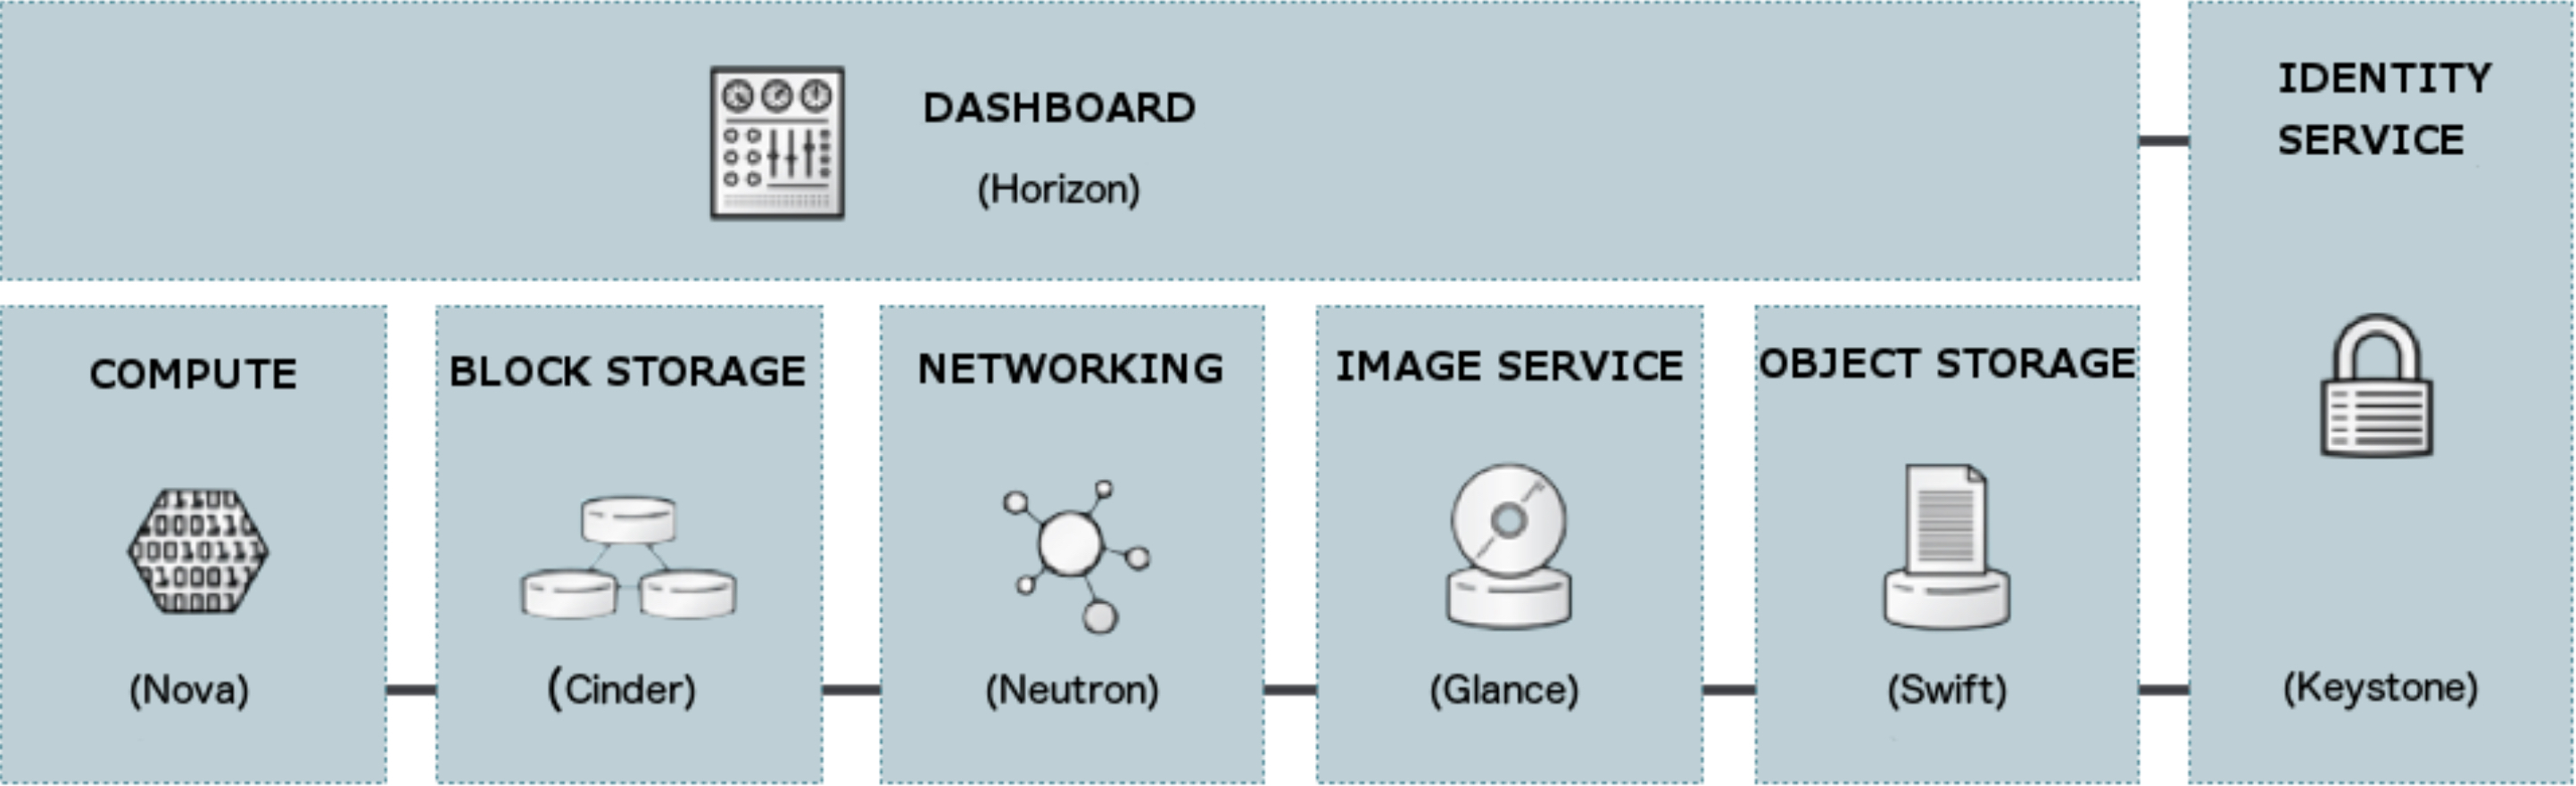
\includegraphics[width=10cm]{Images/OpenStack_Architecture.jpg}
  }{}
  \caption{Architecture of OpenStack}
  \label{fig: OpenStack_Arch_OpenStackDoc}
  \floatfoot{\textit{This architecture shows the basic components of OpenStack for deploying a private, Public, Hybrid cloud using OpenStack}}
  \end{figure}
\subsection{Components of OpenStack}
OpenStack has seven (7) basic components also known as OpenStack projects \cite{OpenStackBlog} as shown in figure in \ref{fig: OpenStack_Arch_OpenStackDoc} that are necessary for deploying a private cloud with OpenStack. It has some other optional components for providing different services for OpenStack users.

\textbf{1. Nova} \\
Nova provides the OpenStack Compute service that supports the management of virtual machine instances that host multi-tiered applications, dev or test environments, “Big Data” crunching Hadoop clusters or high-performance computing. This is possible through an abstraction layer that interfaces with supported hypervisors.

\textbf{2. Swift} \\
Swift provides service for storing and retrieving arbitrary data in the cloud. This service provides both a native API and an Amazon Web Services S3-compatible API. Hence a high degree of resiliency through data replication.

\textbf{3. Cinder} \\
The OpenStack Block Storage service facilitated by Cinder provides persistent block storage for compute instances. It is responsible for managing the life-cycle of block devices, from the creation and attachment of volumes to instances to their release.

\textbf{4. Neutron} \\
IP address management, DNS, DHCP, load balancing, and security groups (network access rules, like firewall policies) is provided by Neutron. It also provides opportunity for software defined networking (SDN). This will allow private cloud owner to manage their guest network configuration, handling common security concerns.

\textbf{5. Horizon} \\
Horizon provides a web-based interface for cloud administration. It allows cloud administrators and tenants to provision, manage, and monitor cloud resources. 

\textbf{6. Keystone} \\
This is the authentication and authorization services provider throughout the entire cloud infrastructure. Security concerns that relates to identity is handled by this component through it's implied service.

\textbf{7. Glance} \\
Glance provides disk-image management services, including image discovery, registration, and delivery services to the Compute service provided by Nova, as needed.

\section{Senlin}
This is a clustering service for OpenStack that creates and operates clusters of common objects made visible by other OpenStack services so as to make the coordination and of this common objects easier. Senlin interacts with OpenStack services via profile plugins that make the resources used by these services open for alterations. This allows Senlin to create, update, delete specific resources. It is designed with the capability of managing different types of objects. 

\begin{figure}[h]
\centering
\IfFileExists{Images/Senlin-architecture.png}{
    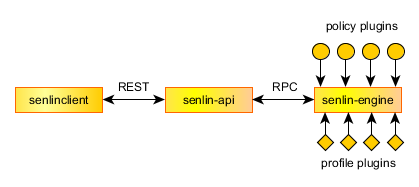
\includegraphics[width=10cm]{Images/Senlin-architecture.png}
  }{}
  \caption{Architecture of Senlin}
  \label{fig: Senlin_Arch_OpenStackDoc}
  \end{figure}

\subsection{Components of Senlin}
\textbf{1. Senlinclient} \\
Senlinclient provides a plugin for the OpenStack client tool that provides command line interface for communicating with the Senlin-api. It aids in managing clusters, nodes, profiles, policies, actions and events.

\textbf{2. Senlin-dashboard} \\
This is a Horizon plugin that provides a user interface for Senlin.

\textbf{3. Senlin-api} \\
This component provides an OpenStack-native REST. It processes API requests by sending them to the Senlin-engine.

\textbf{4. Senlin-engine} \\
This component has the major responsibility of creating and coordinates the clusters, nodes, profiles and policies.

\section{CloudSuite}
The benchmark CloudSuite is a suite for cloud services. With it's third release eight application now have been selected based on their popularity in today’s datacenters \cite{CloudSuiteBlog}. These benchmarks are based on real-world software stacks and represent real-world setups.
\subsection{Benchmarks of CloudSuite}
With the recent release of CloudSuite, the current benchmarks set of CloudSuite now includes: 

\textbf{1. Data Analytics} \\
"The explosion of accessible human-generated information necessitates automated analytical processing to cluster, classify, and filter this information. This benchmark is included in CloudSuite in order to manage the increasing importance of machine learning tasks analyzing large amounts of data in datacenters using the MapReduce framework. It uses Hadoop \cite{hadoop2018} and Mahout\cite{mahout2018}."\cite{CloudSuite_Data_Analytics}

\textbf{2. Data Caching} \\
Data Caching benchmark uses the Memcached \cite{memcached2018} data caching server to measure cloud throughput, expressed as the number of requests served per second (throughput) \cite{CloudSuite_Data_Caching}.

\textbf{3. Data Serving} \\
This benchmark handles the data served in cloud. The framework on which its built comes with appropriate interfaces to populate and stress many popular data serving systems - measuring latency,bandwidth.\\

\textbf{4. Graph Analytics} \\
The CloudSuite graph analytics benchmark performs graph analytics on large-scale datasets. This is done with its graph processing library provided by Apache \cite{apache2018}.

\textbf{5. In-memory Analytics} \\
With explosion of accessible human-generated information the need to cluster, classify and filer information became more important. \cite{klinger2012online}. "This benchmark runs the alternating least squares (ALS) algorithm that is provided by Spark MLlib" \cite{CloudSuite_In-Memory_Analytics}. It measures time in seconds for computing recommendations. This metric is used generally to measure in memory processes in the cloud.

\textbf{6. Web Serving} \\
"Web Serving is a main service in the cloud. Traditional web services with dynamic and static content are moved into the cloud to provide fault-tolerance and dynamic scalability by bringing up the needed number of servers behind a load balancer. Although many variants of the traditional web stack are used in the cloud (substituting Apache with other web server software or using other language interpreters in place of PHP), the underlying service architecture remains unchanged. Independent client requests are accepted by a stateless web server process which either directly serves static files from disk or passes the request to a stateless middleware script, written in a high-level interpreted or byte-code compiled language, which is then responsible for producing dynamic content. All the state information is stored by the middleware in back-end databases such as cloud NoSQL data stores or traditional relational SQL servers supported by key-value cache servers to achieve high throughput and low latency. This benchmark includes a social networking engine (Elgg) and a client implemented using the Faban workload generator. It has four tiers: the web server, the database server, the Memcached server \cite{memcached}, and the clients." \cite{CloudSuite_WebServing}

\textbf{7. Media Streaming} \\
This is a two tier (client and server) benchmark, with server stress as its metrics.

\textbf{8. Web Search}\\
This CloudSuite benchmark measure private cloud response time and throughput. It so much depends on the Apache Solr \cite{apachesoir2018} search engine framework and includes a client machine that simulates real-world clients that send requests to the index nodes.

\section{Scope and Goals}
The exposure of business applications to the web has considerably increased the variability of its workload patterns and volumes as the number of users/customers often grow and shrink at various rates and times. Such characteristics have increasing demand for flexible, yet inexpensive computing infrastructure to accommodate varying workloads. Cloud computing is useful in situations such as this. It is also useful in fields other than business as educational institutions also take advantage of its characteristics to create learning platforms for her students \cite{bora2013learning}. By using cloud computing, they can perform their learning tasks at lower cost.

Although cloud computing is a promising technology, there exist number of open issues that threaten its efficiency: the conception of service contracts, the real economic benefits, the choice of suitable software architecture, data privacy and the adoption of an agile process. Hence in this work, we want to look at how some of these challenges affects a private cloud implemented using OpenStack. Due to the multiple components, in-turn services available with OpenStack private cloud. It is extremely complicated to understand what exactly goes wrong and to locate the bottlenecks without the appropriate benchmark and benchmark tools. To understand this issues more and how to handle it, a powerful component of OpenStack, Ceilometer - that provides monitoring services, will be deployed along side CloudSuite to our private cloud. Ceilometer contains a powerful library osprofiler that is used by all OpenStack projects and their python clients, hence our interest in it. It goes through all involved services and builds a tree of calls making it easy to locate bottlenecks in the private cloud.

Elasticity as a key characteristics of cloud computing allows applications to acquire and release resources dynamically, adjust to changing demands of cloud users. In resource allocation deciding the correct amount of resources is not an easy task and therefore it is most desirable if the system automatically - with minimum or no human intervention, allocates available resources according to the workload handled by the application. This is known as system auto-scaling. It can be horizontal or vertical. Senlin, a clustering service for OpenStack allows for automatic resource allocation.

This work will also study how many virtual machines can be deployed to the private cloud and yet allow optimal running of applications on it. This will be determined by looking at how many requests per second the VM instances can cope with, studied using the Data Caching benchmark of CloudSuite.

This work will also study what the cost effect of using the private cloud for teaching purposes at the chair and also understand what the best configuration for such a cloud model will be. It will also look at auto-scaling in OpenStack, with a deeper dive into auto-scaling issues of the OpenStack.

At the end of this work we will provide an overview of the OpenStack projects/services, test sample configurations, select services to be included in OpenStack private cloud deployment for optimal functionality, deploy a private cloud on the Chair's server, test the use of the services of the private cloud, understand auto-scaling in OpenStack and its issues. We will also provide a documentation of the deployment process, a short user guide for OpenStack and CloudSuite, analyses results based on ran tests and finally make recommendations on how to optimize OpenStack.

\section{Thesis Structure}
This thesis is constructed in the following way; chapter one will be the introduction, here we present the problem along with a brief introduction to OpenStack and CloudSuite. Chapter two will be the literature review and this will consists of the background information that represent the underlying concepts of this thesis. Chapter three will be research methodology detailing the steps taken to deploy the private cloud and set-up the measuring tools. It will also detail the configurations of the cloud and why the chosen configuration/set-up was selected. Chapter four will be Research result, here the results from the measurements will be detailed. In Chapter 5, we will summarize the results and also explain the room for improvement and future work.